\documentclass[conference]{IEEEtran}
\IEEEoverridecommandlockouts
\usepackage{cite}
\usepackage{amsmath,amssymb,amsfonts}
\usepackage{algorithmic}
\usepackage{graphicx}
\usepackage{textcomp}
\usepackage{xcolor}
\usepackage{url}
\usepackage{tikz}
\usetikzlibrary{arrows.meta,positioning}
\def\BibTeX{{\rm B\kern-.05em{\sc i\kern-.025em b}\kern-.08em
    T\kern-.1667em\lower.7ex\hbox{E}\kern-.125emX}}

\begin{document}

\title{Dual-Learning Adaptive Large Neighborhood Search for One-Dimensional Bin Packing:\\
	Online Operator Selection and Offline Learned Repair}

\author{
	\IEEEauthorblockN{Mohamed El Amine Kherroubi, Rayan Boukakiou, Idriss Yacine Ziadi, Idris Himeur, Adem Abdelhafidh Diar}
	\IEEEauthorblockA{\textit{Higher National School of Computer Science (ESI)}\\
		Algiers, Algeria}
}

\maketitle

\begin{abstract}
	The one-dimensional bin packing problem (1D-BPP) is a strongly NP-hard
	combinatorial optimization problem in which a set of weighted items must be
	packed into the fewest identical capacity-limited bins. Metaheuristics scale to
	large instances but rely on hand-designed operators and fixed policies that do
	not adapt to the state of the search. We present a dual-learning Adaptive Large
	Neighborhood Search (ALNS) that injects machine learning at two distinct decision
	points of a single search loop: an \emph{online} warm-start contextual bandit
	(LinUCB) selects the destroy operator from a five-dimensional search-state
	context, while an \emph{offline} gradient-boosted-trees model, trained by
	behavioral cloning of Best-Fit Decreasing, ranks feasible bins during repair. An
	ablation study isolates the contribution of each learning component, and a
	multi-dataset evaluation on standard benchmarks (Scholl, Falkenauer, W\"ascher,
	Hard28) characterizes the combined method. With a budget of $5000$ ALNS
	iterations, all four ablation configurations reach a near-optimal mean gap of
	$0.05$ bins on the Scholl-2 slice ($20$ instances); the two learning
	components affect only solve time on this slice. In the comparative study the
	dual-learning ALNS achieves the best mean gap ($0.05$ bins, versus $0.25$ for
	ant colony optimization at roughly $22\times$ the runtime), dominating every
	classical baseline on quality. Across the five full benchmark families ($685$
	instances) the combined method reaches the optimum on $86\%$ of Scholl-2 and
	$61\%$ of Falkenauer-U instances.
\end{abstract}

\begin{IEEEkeywords}
	bin packing, adaptive large neighborhood search, contextual bandit, LinUCB,
	gradient boosting, hyper-heuristics, machine learning, combinatorial optimization
\end{IEEEkeywords}

\section{Introduction}\label{sec:intro}

The one-dimensional bin packing problem (1D-BPP) is a classical combinatorial
optimization problem with broad industrial relevance, from logistics and
cutting-stock to scheduling and cloud resource allocation. Given $n$ items, each
with a positive integer size, and an unlimited supply of identical bins of fixed
capacity $C$, the task is to assign every item to a bin without exceeding capacity
while using as few bins as possible. Despite its simple statement, 1D-BPP is
strongly NP-hard~\cite{bGarey}, so exact solvers do not scale to large instances
and practitioners rely on heuristics and metaheuristics.

Two families dominate practical 1D-BPP solving. Constructive heuristics such as
First-Fit Decreasing (FFD) and Best-Fit Decreasing (BFD) run in $O(n\log n)$ and
offer bounded worst-case guarantees---FFD uses at most $\tfrac{11}{9}\,\mathrm{OPT}+\tfrac{6}{9}$
bins~\cite{bJohnson}---but they produce a single deterministic packing with no
further improvement. Metaheuristics---simulated annealing~\cite{bKirkpatrick},
tabu search~\cite{bGlover}, grouping genetic algorithms~\cite{bFalkenauer}, and
ant colony optimization~\cite{bDorigo}---explore the solution space iteratively
and reach higher-quality packings on hard instances. Their effectiveness,
however, hinges on manually designed neighborhood operators and on
selection and acceptance policies whose parameters are fixed in advance and
applied identically to every instance and at every stage of the search.
Crucially, classical metaheuristics do not exploit the information generated
during the search itself: neither the time-varying usefulness of an operator nor
the structural regularities of good placements are ever learned.

Machine learning (ML) offers a principled way to make these decisions
data-driven. Following the taxonomy of Bengio \textit{et al.}~\cite{bBengio}, ML
can be hybridized with metaheuristics in three broad modes: (i) predicting
algorithm configuration or parameters offline, (ii) guiding search decisions
online from the current state, and (iii) replacing a hand-crafted operator with a
learned model. The first mode adapts poorly within a single run, and the third
can be data- and compute-intensive in isolation. We therefore combine the second
and third modes at the two decisions that most influence ALNS quality: which part
of the incumbent solution to destroy, and how to rebuild it.

Learning-augmented metaheuristics have shown strong results on routing and
packing problems. Reinforcement learning has been used to select low-level
heuristics in hyper-heuristic frameworks, and neural models have been embedded in
large neighborhood search---for example Neural LNS for vehicle
routing~\cite{bHottung}---to learn destruction or repair policies. Contextual
bandits, in particular LinUCB~\cite{bLi,bChu}, provide a lightweight online
mechanism for adaptive operator selection with theoretical regret guarantees,
while gradient-boosted trees~\cite{bFriedman} are strong tabular rankers
well suited to scoring candidate placements. These ingredients have rarely been
combined within a single bin-packing solver.

This paper presents a dual-learning ALNS for 1D-BPP that injects learning at both
decision points of the destroy--repair loop. First, an online warm-start LinUCB
contextual bandit selects, at every iteration, one of three destroy operators
from a five-dimensional description of the current search state. Second, an
offline gradient-boosted-trees model, trained by behavioral cloning of BFD, ranks
the feasible bins for each displaced item during repair. The two components are
independent and can be toggled separately, which lets us isolate their individual
and joint contributions through an ablation study. To our knowledge, this
two-point integration---online operator selection together with offline learned
repair---has not been reported for bin packing.

The remainder of the paper is organized as follows.
Section~\ref{sec:formulation} formalizes the problem,
Section~\ref{sec:approach} describes the dual-learning ALNS and its two learning
components, Section~\ref{sec:experiments} reports the experimental protocol, the
ablation study, and the multi-dataset and comparative results, and
Section~\ref{sec:conclusion} concludes and outlines perspectives.

\section{Problem Formulation}\label{sec:formulation}

Let $\mathcal{I}=\{1,\dots,n\}$ be a set of items with strictly positive integer
sizes $s_i\in\mathbb{Z}_{>0}$, and let identical bins have integer capacity
$C\in\mathbb{Z}_{>0}$ with $s_i\le C$ for all $i$. Using binary variables
$x_{ij}=1$ iff item $i$ is placed in bin $j$, and $y_j=1$ iff bin $j$ is used
(with $j\in\{1,\dots,n\}$), the problem is:
\begin{align}
	\min \quad       & \sum_{j=1}^{n} y_j \label{eq:obj}                                                     \\
	\text{s.t.}\quad & \sum_{j=1}^{n} x_{ij}=1,               &  & \forall i\in\mathcal{I} \label{eq:assign} \\
	                 & \sum_{i=1}^{n} s_i\,x_{ij}\le C\,y_j,  &  & \forall j \label{eq:cap}                  \\
	                 & x_{ij}\le y_j,\; x_{ij},y_j\in\{0,1\}. &  & \label{eq:link}
\end{align}
Constraint~\eqref{eq:assign} assigns each item to exactly one bin,
\eqref{eq:cap} enforces capacity and links assignment to bin usage, and the
objective~\eqref{eq:obj} minimizes the number of bins used. A standard continuous
lower bound is
\begin{equation}
	\mathrm{LB}_1=\left\lceil \frac{\sum_{i=1}^{n} s_i}{C} \right\rceil ,\label{eq:lb}
\end{equation}
which is valid because the total item volume $\sum_i s_i$ must be distributed over
bins of capacity $C$, requiring at least $\sum_i s_i / C$ of them; integrality
gives the ceiling. Sharper bounds exist, such as the $L_2$ bound of Martello and
Toth~\cite{bMartello}, but $\mathrm{LB}_1$ is sufficient as the progress indicator
used throughout this work. 1D-BPP is strongly NP-hard by reduction from
3-Partition~\cite{bGarey}, which justifies a metaheuristic treatment.

\section{Proposed Dual-Learning ALNS}\label{sec:approach}

\begin{figure}[t]
	\centering
	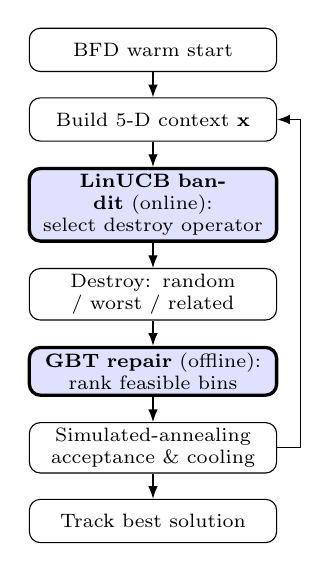
\begin{tikzpicture}[
		node distance=3.2mm,
		box/.style={draw, rounded corners, align=center, font=\scriptsize,
				minimum height=5.5mm, text width=3.0cm, inner sep=2pt},
		ml/.style={box, fill=blue!12, very thick},
		arr/.style={-{Latex[length=1.6mm]}}
		]
		\node[box] (start) {BFD warm start};
		\node[box, below=of start] (ctx) {Build 5-D context $\mathbf{x}$};
		\node[ml, below=of ctx] (bandit) {\textbf{LinUCB bandit} (online):\\ select destroy operator};
		\node[box, below=of bandit] (destroy) {Destroy: random / worst / related};
		\node[ml, below=of destroy] (repair) {\textbf{GBT repair} (offline):\\ rank feasible bins};
		\node[box, below=of repair] (sa) {Simulated-annealing\\ acceptance \& cooling};
		\node[box, below=of sa] (best) {Track best solution};
		\foreach \a/\b in {start/ctx, ctx/bandit, bandit/destroy, destroy/repair, repair/sa, sa/best}
		\draw[arr] (\a)--(\b);
		\draw[arr] (sa.east) -- ++(3mm,0) |- (ctx.east);
	\end{tikzpicture}
	\caption{Architecture of the dual-learning hybrid ALNS. Shaded boxes mark the two
		machine-learning injection points; the right-hand arrow is the iteration loop.}
	\label{fig:arch}
\end{figure}

\subsection{Solution Encoding and Warm Start}
A solution is the assignment of items to bins. Internally the search stores, for
each item, the index of its bin and, for each bin, its current load, so that a
removal or insertion updates in $O(1)$ and the objective---the number of
non-empty bins---is read directly. The search is warm-started with Best-Fit
Decreasing (BFD): items are processed in non-increasing size order and each is
placed in the open bin that leaves the smallest residual capacity, a new bin being
opened only when no bin can host it. A tight initial packing gives ALNS fewer bins
to eliminate and shortens the time spent recovering from a poor initialization.

\subsection{Adaptive Large Neighborhood Search}
The search follows the large-neighborhood-search paradigm~\cite{bShaw} in its
adaptive form~\cite{bRopke}. Each iteration (i) \emph{destroys} the incumbent by
removing a subset $D$ of items and (ii) \emph{repairs} the partial solution by
reinserting $D$. Because repair can produce any feasible completion, the
neighborhood is implicitly exponential in $|D|$, which allows the search to escape
local optima unreachable by single-item moves. Three destroy operators form the
portfolio: \emph{random} removal of $k$ items; \emph{worst-load} removal, which
empties the least-filled bins first; and \emph{related-item} removal, which
removes a seed item together with the items closest to it in size. The destruction
radius $k$ is drawn uniformly from $[\lfloor 0.05\,n\rfloor,\lfloor 0.25\,n\rfloor]$
and is widened toward its upper bound as stagnation grows; all operators guarantee
that at least one item remains placed, preventing total destruction.

\subsection{Acceptance: Simulated Annealing}
Candidates are accepted by simulated annealing. A candidate whose bin-count change
is $\Delta$ is accepted whenever $\Delta\le 0$, and otherwise with probability
$\exp(-\Delta/T)$. The temperature follows geometric cooling
$T\leftarrow \alpha_{\mathrm{cool}}\,T$ with $T_0=1/\ln 2$ and
$\alpha_{\mathrm{cool}}=0.9995$. To avoid premature freezing, a soft reheat lifts
$T$ back toward $0.35\,T_0$ during prolonged stagnation, and a diversification
restart---reverting to the best solution found, partially reheating to
$0.20\,T_0$, and shrinking the patience window---is triggered when no improvement
occurs within a budget of iterations. The fixed iteration budget is the sole
termination criterion.

\subsection{Online Learning: Warm-Start LinUCB Operator Selection}
Operator selection is delegated to a warm-start contextual bandit. During the
first $300$ selections, a context-free Beta--Bernoulli Thompson sampler quickly
identifies promising operators, mitigating the cold-start of a linear bandit on
short runs. Thereafter a disjoint LinUCB bandit~\cite{bChu} takes over: for a
context vector $\mathbf{x}\in\mathbb{R}^5$ it selects the operator that maximizes
\begin{equation}
	\hat{\boldsymbol{\theta}}_k^\top \mathbf{x}
	+ \alpha\sqrt{\mathbf{x}^\top A_k^{-1}\mathbf{x}},
	\qquad \hat{\boldsymbol{\theta}}_k=A_k^{-1}\mathbf{b}_k,\label{eq:ucb}
\end{equation}
with $\alpha=0.3$, updating $A_k^{-1}$ by the $O(d^2)$ Sherman--Morrison formula
and $\mathbf{b}_k$ by $\mathbf{b}_k\leftarrow\mathbf{b}_k+r\,\mathbf{x}$. The
context encodes the normalized temperature $T/T_0$, the stagnation progress toward
the next restart, the cost-to-bound ratio $f(x)/\mathrm{LB}_1$, the destruction
radius $k/n$, and the overall search progress. The reward is
$\min(1,\,\text{bins\_saved}/\text{gap})$ when bins are saved---normalized by the
gap to $\mathrm{LB}_1$ so that improvements near the optimum count more---$0.2$ for
an accepted non-improving move, and $0$ for a rejected one.

\subsection{Offline Learning: GBT Repair by Behavioral Cloning}
Repair reinserts displaced items in non-increasing size order. For an item, the
set of feasible bins (those with enough residual capacity) is scored by a gradient
boosted classifier~\cite{bFriedman}, and the item is placed in the highest-scoring
bin; a new bin is opened only when no bin is feasible. The model is trained offline
by behavioral cloning of BFD: each feasible (item, bin) pair is labeled $1$ if BFD
would select that bin and $0$ otherwise. Every pair is encoded by eleven features
normalized by capacity or instance size---item size and its square, size rank,
fraction of items still to reinsert, bin load, residual capacity, post-placement
slack, bin occupancy, the largest and smallest item already in the bin, and the
fill ratio. Training pools two trace types---fresh BFD replays and
post-destruction repair states---to reduce the distribution shift between offline
replay and the mid-search states encountered at inference. A standard scaler is
stored with the model, and a fast predictor applies it in NumPy and reads class
probabilities directly, avoiding per-call validation overhead. Algorithm~\ref{alg:alns}
summarizes the complete loop.

\subsection{Parameter Tuning}

The hybrid ALNS exposes nine tunable metaheuristic knobs that govern the cooling
schedule, destruction radius, reheat and restart thresholds, and bandit
exploration (Table~\ref{tab:tuning-params}). These parameters interact
non-trivially --- a faster cooling rate may be compensated by more aggressive
reheating, and the optimal destruction radius depends on the stagnation budget.
Manual or grid-based tuning of all nine dimensions is brittle and does not
generalise across datasets.  We therefore design a three-stage automated pipeline
powered by Optuna~\cite{bAkiba} that progressively focuses the search from wide
exploration to fine-grained refinement.

\begin{table}[htbp]
\caption{The nine tunable hyperparameters.  Stage~1 ranges define the full
coarse search space; Stage~2 windows are computed dynamically as $\pm15$--$25\%$
of the Stage~1 best.  Log-scale sampling is used where the effect spans orders
of magnitude.}
\label{tab:tuning-params}
\centering
\small
\begin{tabular}{l c c c}
\hline
\textbf{Parameter} & \textbf{Default} & \textbf{Stage~1 range} & \textbf{Role} \\
\hline
$\alpha_{\mathrm{cool}}$ & $0.9995$ & $(0.998,\;0.9999)$ & SA geometric cooling factor \\
$\mathrm{bandit\_alpha}$ & $0.30$ & $(0.05,\;1.0)\;\text{log}$ & LinUCB exploration bonus \\
$\mathrm{initial\_temperature}$ & $1/\ln 2$ & $(0.5,\;5.0)\;\text{log}$ & SA starting temperature \\
$k_{\min}$ & $0.05\,n$ & $(0.01n,\;0.20n)$ & Min destruction radius \\
$k_{\max}$ & $0.25\,n$ & $(0.10n,\;0.40n)$ & Max destruction radius \\
$\mathrm{no\_improve\_frac}$ & $0.05$ & $(0.01,\;0.20)$ & Stagnation budget fraction \\
$\mathrm{reheat\_soft\_mult}$ & $0.35$ & $(0.10,\;0.90)$ & Soft-reheat temperature multiplier \\
$\mathrm{reheat\_hard\_mult}$ & $0.20$ & $(0.05,\;0.80)$ & Hard-restart temperature multiplier \\
$\mathrm{warmup\_calls}$ & $300$ & $[50,\;600]$ & TS warm-up length before LinUCB \\
\hline
\end{tabular}
\end{table}

\subsubsection{Composite Objective}

Every candidate configuration is evaluated on a fixed bank of $100$ bin-packing
instances (see below), and scored by a composite objective that balances solution
quality against computational cost:

\begin{equation}
\label{eq:composite}
\Phi(\theta) \;=\;
w_q \cdot \frac{1}{N}\sum_{i=1}^{N} \frac{b_i(\theta) - \mathrm{LB}_{1,i}}{\max(\mathrm{LB}_{1,i},1)}
\;+\;
w_t \cdot \frac{1}{N}\sum_{i=1}^{N} \frac{t_i(\theta)}{\max(\tau,10^{-9})},
\end{equation}

\noindent where $b_i(\theta)$ is the bin count produced by configuration $\theta$
on instance $i$, $\mathrm{LB}_{1,i}$ is the continuous lower bound
(\ref{eq:lb}), $t_i(\theta)$ is the wall-clock time, $\tau=60$\,s is the
time-normalisation constant, and $N=100$.  The weights $w_q=0.9$,
$w_t=0.1$ reflect that solution quality is the primary concern but a non-zero
time component is essential to prevent the optimiser from selecting
impractically slow (e.g., overly exploratory) configurations.  The relative gap
formulation renders the quality metric scale-invariant across instances of
different optimal bin counts, and the $\max$ guards protect against degenerate
division.

\subsubsection{Instance Bank}

To ensure that tuning signal generalises across problem sizes and dataset
structures, the evaluation bank samples $100$ instances from the combined
pool of five benchmark families via strided, jittered selection: Falkenauer-T
(5 instances), Falkenauer-U (40), Scholl-1 (10), Scholl-2 (35), and Scholl-3
(10).  The same bank is reused for every evaluation, giving every candidate a
deterministic ranking.  A smaller $20$-instance stratified subset serves the
isolation step (Stage~0) for computational efficiency.

\subsubsection{Three-Stage Pipeline}

\paragraph{Stage~0: Isolation Grid Search.}
Rather than submitting all nine parameters directly to a Bayesian optimiser, we
first disentangle them into three independent groups and perform a grid search
on each group while holding the others at their defaults.  The three groups are:
(i)~SA thermal parameters (initial temperature, cooling rate, soft and hard
reheat multipliers); (ii)~destruction parameters (min and max destruction
radius, stagnation budget); and (iii)~bandit parameters (exploration coefficient
$\alpha$, warm-up length).  To prevent the bandit's online adaptivity from
confounding the measurement of a group's standalone effect, the destroy operator
is forced to uniform random throughout every isolation evaluation
(\texttt{force\_uniform\_random=True}).

Each group is searched over a small Cartesian grid of $3$ values per dimension
--- $54$ valid configurations for the SA group (after imposing the constraint
$\mathrm{reheat\_hard} < \mathrm{reheat\_soft}$, which encodes the design
principle that a diversification restart must apply a stronger cooldown than a
periodic soft reheat), $24$ for the destruction group (filtering
$k_{\max} \leq k_{\min}$), and $9$ for the bandit group.  Every grid point is
evaluated on the $20$-instance isolation bank at $2\,000$ ALNS iterations.  The
best configuration from each group is merged into a single ``after-isolation''
anchor.

Critically, the isolation anchor is \emph{not} used to shrink the search ranges
of the subsequent stage.  Instead it is enqueued via
\texttt{study.enqueue\_trial()} so that the TPE surrogate model receives an
additional known-good observation from which to learn.  The range boundaries of
Stage~1 remain the full, wide $S_1$ intervals.  This is the fundamental
distinction between the isolation-to-Stage~1 handoff and the Stage~1-to-Stage~2
handoff: the former provides a training point without restricting the search
domain; the latter physically contracts the domain.

\paragraph{Stage~1: Coarse Bayesian Search.}
Stage~1 deploys Optuna's Tree-structured Parzen Estimator (TPE) over the full
$S_1$ search space (Table~\ref{tab:tuning-params}, Column~3).  TPE constructs a
probabilistic surrogate model by comparing the density of good versus poor
trials, favouring regions where promising configurations concentrate.  Ten
warm-up trials seed the model before the acquisition function drives the
remaining draws.  The default configuration is always enqueued as trial~0 to
give the surrogate an absolute reference point; the isolation anchor occupies
trial~1 when available.

Two domain constraints are enforced at the objective level via
\texttt{optuna.TrialPruned()}: trials proposing $k_{\min} \geq k_{\max}$ or
$\mathrm{reheat\_hard} \geq \mathrm{reheat\_soft}$ are pruned before
consuming evaluation budget.  This avoids wasting compute on parameter
combinations that violate the structural logic of the solver.  At $5\,000$ ALNS
iterations per instance and $N=100$ instances per trial, the Stage~1 budget is
$50$ trials.

\paragraph{Stage~2: Fine Bayesian Search.}
Stage~2 refines within the most promising basin identified by Stage~1.  The
search ranges are \emph{physically narrowed} to a window centred on the
Stage~1 best value for each parameter.  Parameters whose effects are
scale-free receive multiplicative offsets: $\pm15$--$25\%$ of the anchor value.
Parameters with narrow or integer domains receive additive offsets (e.g.,
$\pm0.02$ for $k_{\min}$).  Upper bounds are clamped by solver-imposed limits
where necessary --- in particular $\alpha_{\mathrm{cool}} < 1.0$ --- to prevent
the offset arithmetic from producing values that the solver would reject.

The anchor --- the Stage~1 best merged with defaults --- is enqueued as trial~0.
The default configuration is deliberately \emph{not} re-enqueued: Stage~2 trusts
the basin found in Stage~1 and would gain no signal from the distant default.
TPE operates within the narrow window for $50$ trials at $5\,000$ iterations per
instance.

\paragraph{Final Evaluation.}
After Stage~2, the best-found configuration is re-evaluated on the full
$100$-instance bank at $5\,000$ iterations, producing an apples-to-apples
comparison against the baseline default (evaluated identically at the start of
the pipeline).  All structural parameters listed in
Table~\ref{tab:tuning-params} are held fixed at their default values throughout
every stage; they constitute safety floors and design constants whose joint
tuning with the metaheuristic knobs would dilute the optimiser's signal and
unnecessarily expand the search dimensionality.

\begin{figure}[t]
	\centering
	\begin{algorithmic}[1]
		\STATE $x \leftarrow \textsc{BFD-WarmStart}()$;\; $x^\star \leftarrow x$
		\FOR{$t=1$ \TO $\mathrm{max\_iter}$}
		\STATE $\mathbf{x}_{\text{ctx}} \leftarrow \textsc{Context}(x,T,t)$
		\STATE $a \leftarrow \textsc{Bandit.Select}(\mathbf{x}_{\text{ctx}})$
		\STATE $(\hat{x},D) \leftarrow \textsc{Destroy}_a(x,k)$
		\STATE $x' \leftarrow \textsc{RepairGBT}(\hat{x},D)$
		\STATE accept $x'$ by simulated annealing; update $x^\star$
		\STATE $\textsc{Bandit.Update}(a,\mathbf{x}_{\text{ctx}},r)$;\; cool/reheat $T$
		\ENDFOR
		\RETURN $x^\star$
	\end{algorithmic}
	\caption{Dual-learning hybrid ALNS.}
	\label{alg:alns}
\end{figure}


\section{Experiments, Results and Analysis}\label{sec:experiments}

\subsection{Protocol and Setup}
All runs use a fixed random seed ($42$), a budget of $5000$ ALNS iterations, an
initial temperature $T_0=1/\ln 2$, a cooling rate $\alpha_{\mathrm{cool}}=0.9995$,
and a single pre-trained repair model shared across every dataset. The solver is
implemented in Python~3.13 with scikit-learn~\cite{bPedregosa} for the
gradient-boosted repair model, and experiments were run on a workstation running
Windows~11 with an Intel Core i9-13950HX CPU and 64\,GB of RAM. Solution quality
is measured by the gap to the
lower bound, $\text{gap}=\text{bins used}-\mathrm{LB}_1$ of~\eqref{eq:lb}; a gap of
zero certifies optimality with respect to $\mathrm{LB}_1$.

\subsection{Datasets}
We evaluate on four widely used 1D-BPP benchmark families, summarized in
Table~\ref{tab:datasets}. Scholl-2 contains uniformly distributed instances with
capacity $1000$ and $50$--$500$ items. Falkenauer-T comprises triplet instances,
where an optimal bin holds one large and two small items, at capacity $1000$.
Falkenauer-U holds uniform instances with the tighter capacity $150$. W\"ascher
contributes hard cutting-stock-style instances at capacity $10000$, and Hard28 a
set of difficult $160$--$200$-item instances at capacity $1000$.

\begin{table}[htbp]
	\caption{Benchmark datasets used in the evaluation.}
	\label{tab:datasets}
	\centering
	\begin{tabular}{l c c l}
		\hline
		\textbf{Dataset} & \textbf{Capacity} & \textbf{Items} & \textbf{Structure} \\
		\hline
		Scholl-2         & 1000              & 50--500        & uniform            \\
		Falkenauer-T     & 1000              & 60--501        & triplets           \\
		Falkenauer-U     & 150               & 120--1000      & uniform            \\
		W\"ascher        & 10000             & varied         & cutting-stock      \\
		Hard28           & 1000              & 160--200       & hard               \\
		\hline
	\end{tabular}
\end{table}

\subsection{Ablation Study}
To isolate the effect of each learning component we run four configurations on
the first $20$ Scholl-2 $50$-item instances, keeping all ALNS settings identical
and toggling only the two switches (Table~\ref{tab:ablation},
Fig.~\ref{fig:ablation}). With a $5000$-iteration budget all four configurations
reach the same near-optimal mean gap of $0.05$ bins on this slice, so the
contributions of the two learning components are visible only in solve
\emph{time}, not in solution quality. The no-learning baseline---random operator
choice and best-fit repair---is the fastest at $3.14$\,s. Enabling the online
bandit alone adds only $0.07$\,s, while enabling the offline repair model adds
$5.82$\,s, so the per-placement scoring of the repair model dominates the cost.
On this small, near-optimal slice the learning components add overhead without
quality gain; their benefit is expected on harder instances with larger
feasible-bin sets, where the offline model can distinguish placements that
best-fit repair cannot (Tables~\ref{tab:multi} and~\ref{tab:compare}).

\begin{table}[htbp]
	\caption{Ablation on Scholl-2 (50 items, 20 instances).}
	\label{tab:ablation}
	\centering
	\begin{tabular}{l c c c c}
		\hline
		\textbf{Configuration} & \textbf{Avg bins} & \textbf{Avg gap} & \textbf{Fill (\%)} & \textbf{Time (s)} \\
		\hline
		No learning            & 17.4              & 0.05             & 95.84              & 3.136             \\
		Online only            & 17.4              & 0.05             & 95.84              & 3.208             \\
		Offline only           & 17.4              & 0.05             & 95.84              & 8.954             \\
		Both combined          & 17.4              & 0.05             & 95.84              & 8.950             \\
		\hline
	\end{tabular}
\end{table}

\begin{figure}[t]
	\centering
	
\includegraphics[width=0.92\linewidth]{figures/ablation.png}
	\caption{Ablation on Scholl-2 ($5000$ iterations, $20$ instances): the four
		configurations reach the same near-optimal mean gap ($0.05$); the offline
		repair model adds about $5.8$\,s of per-placement scoring without quality
		gain on this slice.}
	\label{fig:ablation}
\end{figure}

\subsection{Multi-Dataset Results}
Table~\ref{tab:multi} reports the combined method across the five \emph{full}
benchmark families ($685$ instances in total) with per-instance time limits scaled
to a $5000$-iteration budget. The solver reaches $\mathrm{LB}_1$ on $86\%$ of
Scholl-2 instances (mean gap $0.28$) and $61\%$ of Falkenauer-U instances (mean
gap $0.45$). The triplet instances of Falkenauer-T are the hardest relative to
$\mathrm{LB}_1$ (mean gap $1.06$, no optimum reached), consistent with the known
weakness of the continuous bound on triplet structures, where the true optimum
typically exceeds $\mathrm{LB}_1$ by one bin. Mean runtime grows steeply with
item count---about $33$\,s on Scholl-2 but more than $1200$\,s on the
$160$--$200$-item Hard28 family---reflecting the cost of model-guided repair over
larger feasible-bin sets at $5000$ iterations. Instances that exceeded their
per-instance time budget are reported with the solver's best result at the
deadline, an honest upper bound rather than the lower bound.

\begin{table}[htbp]
	\caption{Combined method across the five full datasets (685 instances total) with per-instance time limits.}
	\label{tab:multi}
	\centering
	\begin{tabular}{l c c c c}
		\hline
		\textbf{Dataset}  & \textbf{N} & \textbf{Avg gap} & \textbf{Opt (\%)} & \textbf{Avg time (s)} \\
		\hline
		Scholl-2          & 480        & 0.28             & 85.8              & 33.37                 \\
		Falkenauer-T      & 80         & 1.06             & 0.0               & 53.48                 \\
		Falkenauer-U      & 80         & 0.45             & 61.3              & 541.49                \\
		W\"ascher         & 17         & 0.82             & 17.6              & 28.39                 \\
		Hard28            & 28         & 0.82             & 17.9              & 1286.82               \\
		\hline
	\end{tabular}
\end{table}

\subsection{Comparative Study}
Table~\ref{tab:compare} compares the dual-learning ALNS with classical baselines
implemented in the same framework, all run in a single session on the hardware
above so that runtimes are directly comparable. Exact methods (branch-and-bound,
dynamic programming) are omitted because they are intractable at $n=50$. The pure
constructive heuristics FFD and BFD are instantaneous but leave a mean gap of
$1.40$ bins, and the standalone trajectory metaheuristics---simulated annealing
and tabu search---do not improve on construction within their default budgets on
this slice. The population methods are stronger: the genetic algorithm reaches a
mean gap of $0.90$ in $1.11$\,s and ant colony optimization $0.25$ in
$193.91$\,s. The dual-learning ALNS attains the best mean gap of $0.05$ in
$8.64$\,s, dominating every baseline on quality while running about $22\times$
faster than ant colony optimization. The metaheuristic baselines are stochastic,
so their gaps vary across runs; a single aligned run is reported.

\begin{table}[htbp]
	\caption{Comparison on Scholl-2 (50 items, 20 instances): mean gap to $\mathrm{LB}_1$ and mean solve time.}
	\label{tab:compare}
	\centering
	\begin{tabular}{l c c}
		\hline
		\textbf{Method}             & \textbf{Avg gap} & \textbf{Time (s)} \\
		\hline
		FFD / BFD                   & 1.40             & $<0.01$           \\
		Simulated annealing         & 1.40             & 0.33              \\
		Tabu search                 & 1.40             & 0.22              \\
		Genetic algorithm           & 0.90             & 1.11              \\
		Ant colony                  & 0.25             & 193.91            \\
		\textbf{Dual-learning ALNS} & \textbf{0.05}    & \textbf{8.64}     \\
		\hline
	\end{tabular}
\end{table}

\section{Conclusion and Perspectives}\label{sec:conclusion}
We presented a dual-learning Adaptive Large Neighborhood Search for the
one-dimensional bin packing problem that injects machine learning at two decision
points of the destroy--repair loop: an online warm-start LinUCB bandit for
destroy-operator selection and an offline gradient-boosted repair model trained by
behavioral cloning of Best-Fit Decreasing. An ablation isolating the two
components shows that with a $5000$-iteration budget all four configurations
reach the same near-optimal mean gap of $0.05$ bins on the Scholl-2 slice, so
the contributions of the two learning components are visible there only as
solve-time overhead. On the comparative study the dual-learning configuration
achieves the best gap ($0.05$), dominating every baseline on quality while
running about $22\times$ faster than ant colony optimization. Across the five
full benchmark families ($685$ instances) the combined method reaches the
optimum on $86\%$ of Scholl-2 and $61\%$ of Falkenauer-U instances; harder
families remain bounded by the per-instance time budget. The main limitations
are the single-run reporting of stochastic baselines and the runtime overhead
of the offline model on the largest instances. Future work will extend the evaluation to full datasets and stronger
lower bounds such as the Martello--Toth $L_2$ bound, where learned repair is
expected to pay off on larger feasible-bin sets, replace the cloned repair model
with a policy learned directly from search reward, and study the transfer of the
learned components across instance families.

\begin{thebibliography}{00}
	\bibitem{bCoffman} E. G. Coffman, M. R. Garey, and D. S. Johnson, ``Approximation algorithms for bin packing: a survey,'' in \textit{Approximation Algorithms for NP-Hard Problems}, 1996, pp. 46--93.
	\bibitem{bDelorme} M. Delorme, M. Iori, and S. Martello, ``Bin packing and cutting stock problems: Mathematical models and exact algorithms,'' \textit{Eur. J. Oper. Res.}, vol. 255, no. 1, pp. 1--20, 2016.
	\bibitem{bJohnson} D. S. Johnson, ``Near-optimal bin packing algorithms,'' Ph.D. dissertation, MIT, Cambridge, MA, 1973.
	\bibitem{bGarey} M. R. Garey and D. S. Johnson, \textit{Computers and Intractability: A Guide to the Theory of NP-Completeness}. San Francisco, CA: Freeman, 1979.
	\bibitem{bMartello} S. Martello and P. Toth, \textit{Knapsack Problems: Algorithms and Computer Implementations}. New York, NY: Wiley, 1990.
	\bibitem{bKirkpatrick} S. Kirkpatrick, C. D. Gelatt, and M. P. Vecchi, ``Optimization by simulated annealing,'' \textit{Science}, vol. 220, no. 4598, pp. 671--680, 1983.
	\bibitem{bGlover} F. Glover, ``Future paths for integer programming and links to artificial intelligence,'' \textit{Comput. Oper. Res.}, vol. 13, no. 5, pp. 533--549, 1986.
	\bibitem{bFalkenauer} E. Falkenauer, ``A hybrid grouping genetic algorithm for bin packing,'' \textit{J. Heuristics}, vol. 2, no. 1, pp. 5--30, 1996.
	\bibitem{bDorigo} M. Dorigo and T. St\"utzle, \textit{Ant Colony Optimization}. Cambridge, MA: MIT Press, 2004.
	\bibitem{bShaw} P. Shaw, ``Using constraint programming and local search methods to solve vehicle routing problems,'' in \textit{Proc. Int. Conf. Principles and Practice of Constraint Programming (CP)}, 1998, pp. 417--431.
	\bibitem{bRopke} S. Ropke and D. Pisinger, ``An adaptive large neighborhood search heuristic for the pickup and delivery problem with time windows,'' \textit{Transp. Sci.}, vol. 40, no. 4, pp. 455--472, 2006.
	\bibitem{bLi} L. Li, W. Chu, J. Langford, and R. E. Schapire, ``A contextual-bandit approach to personalized news article recommendation,'' in \textit{Proc. 19th Int. Conf. World Wide Web (WWW)}, 2010, pp. 661--670.
	\bibitem{bChu} W. Chu, L. Li, L. Reyzin, and R. E. Schapire, ``Contextual bandits with linear payoff functions,'' in \textit{Proc. 14th Int. Conf. Artificial Intelligence and Statistics (AISTATS)}, 2011, pp. 208--214.
	\bibitem{bFriedman} J. H. Friedman, ``Greedy function approximation: a gradient boosting machine,'' \textit{Ann. Statist.}, vol. 29, no. 5, pp. 1189--1232, 2001.
	\bibitem{bBengio} Y. Bengio, A. Lodi, and A. Prouvost, ``Machine learning for combinatorial optimization: a methodological tour d'horizon,'' \textit{Eur. J. Oper. Res.}, vol. 290, no. 2, pp. 405--421, 2021.
	\bibitem{bHottung} A. Hottung and K. Tierney, ``Neural large neighborhood search for the capacitated vehicle routing problem,'' in \textit{Proc. 24th Eur. Conf. Artificial Intelligence (ECAI)}, 2020, pp. 443--450.
	\bibitem{bScholl} A. Scholl, R. Klein, and C. J\"urgens, ``BISON: A fast hybrid procedure for exactly solving the one-dimensional bin packing problem,'' \textit{Comput. Oper. Res.}, vol. 24, no. 7, pp. 627--645, 1997.
	\bibitem{bSchwerin} P. Schwerin and G. W\"ascher, ``The bin-packing problem: A problem generator and some numerical experiments with FFD packing and MTP,'' \textit{Int. Trans. Oper. Res.}, vol. 4, no. 5--6, pp. 377--389, 1997.
	\bibitem{bPedregosa} F. Pedregosa \textit{et al.}, ``Scikit-learn: Machine learning in Python,'' \textit{J. Mach. Learn. Res.}, vol. 12, pp. 2825--2830, 2011.
\bibitem{bAkiba} T. Akiba \textit{et al.}, ``Optuna: A next-generation hyperparameter optimization framework,'' in \textit{Proc. 25th ACM SIGKDD Int. Conf. Knowledge Discovery and Data Mining (KDD)}, 2019, pp. 2623--2631.
\end{thebibliography}

\end{document}
